\title{QR and Least-Squares}
\subtitle{\SubTitleName}
\institute[]{\Course}
\author{\Instructor}
\maketitle   


\begin{frame}\frametitle{Topics and Objectives}
\Emph{Topics} \\
%\TopicStatement
\begin{itemize}

    \item the use of the QR decomposition to solve least-squares problems
    % \item Different methods to solve Least-Squares Problems
    
\end{itemize}

\vspace{0.5cm}

\Emph{Learning Objectives}\\

\begin{itemize}

    \item apply the QR decomposition to solve the normal equations
  
\end{itemize}

\vspace{0.25cm} 
 
 \end{frame}

\begin{frame}{Motivating Questions}

    The normal equations give us a method for calculating a least-squares solution, $\widehat x$. 
    $$
        A ^{T} A \widehat x = A ^{T} \vec b
    $$
    \begin{itemize}
        \item<2-> These equations are often used in situations where $A$ and $\vec b$ are constructed using measured data that contain errors.
        \item<3-> The QR decomposition is often used to reduce the impact of these errors in calculating $\widehat x$. 
    \end{itemize}
    

\end{frame}








\begin{frame}{The QR Factorization for Least-Squares}
\begin{center}\begin{tikzpicture} \node [mybox](box){\begin{minipage}{0.9\textwidth}\vspace{4pt}
     If $A \in \mathbb R^{m \times n}$ has linearly independent columns, then $A = QR$, and for every $ \vec b\in \mathbb R ^{m}$, $ A \vec x=\vec b$ has the unique least-squares solution \onslide<2->{
        \begin{equation*}
            R\widehat x =  Q ^{T} \vec b.
        \end{equation*}}
    \vspace{-12pt}
    \end{minipage}};
    \node[fancytitle, right=10pt] at (box.north west) {Theorem (Least-Squares and $QR$)};
    \end{tikzpicture} \end{center} 
    
    \onslide<4->{Note that $R$ is invertible and upper triangular. So $R\widehat x =  Q ^T \vec b$ may be solved with back-substitution.}
    
\end{frame}



\begin{frame}{Short Proof that $R\widehat x =  Q ^{T} \vec b$}
    
    We can solve the normal equations using:
    \onslide<2->{
    \begin{equation*}
        R\widehat x =  Q ^{T} \vec b.
    \end{equation*}}
    \onslide<3->{Why? If $A = QR$, and the normal equations are $A ^{T} A \widehat x = A ^{T} \vec b$, then}
    \begin{align*}
        \onslide<4->{(QR)^T QR \, \widehat x &= (QR)^T \vec b }\\
        \onslide<5->{R^T Q^TQR \, \widehat x &= R^T Q^T \vec b, \quad \text{but } Q^TQ = I } \\
        \onslide<6->{R^T R \, \widehat x &= R^T Q^T \vec b, \quad \text{but } R \text{ is invertible}}\\
        \onslide<7->{ R \, \widehat x &= Q^T \vec b}
    \end{align*}
    
\end{frame}


\begin{frame}{Process of Using QR to Solve a Least-Squares Problem}

    Given $A$ and $\vec b$, we can use the following process to compute the least-squares solution, $\widehat x$, with the QR decomposition. 
    \vspace{8pt}
    \begin{enumerate}\setlength{\itemsep}{8pt}
        \item<2-> construct QR decomposition of $A$
        \vspace{6pt}
        
        \begin{enumerate}\setlength{\itemsep}{6pt}
            \item<3->[a)] {\normalsize obtain orthonormal basis for $\Col A$ (can use Gram-Schmidt)}
            \item<4->[b)] {\normalsize obtain $Q$ from the orthonormal basis}
            \item<5->[c)] {\normalsize obtain $R$ using $R = Q^TA$}
        \end{enumerate}
        \item<6-> solve $R\widehat x = Q^T\vec b$ to obtain $\widehat x$
    \end{enumerate}
    
\end{frame}
    

\begin{frame}{Applying QR to Solve an Inconsistent System}

    Suppose we are given the data below. 
    
    \pause 
    \vspace{4pt}
    
    \begin{minipage}{0.5\textwidth}
        \onslide<2->{
        \begin{center}
        \begin{tabular}{c|ccccc} 
             $ x$ & $-2$ & $-1$  & $0$ & $1$ & $2$ 
            \\ \hline 
            $ y$ & $-2$ & $-1$  & $1$ & $2$  & $2$
        \end{tabular}
    \end{center}
    }
    \end{minipage} \begin{minipage}{0.45\textwidth}
        \qquad
        \begin{center}
        \onslide<3->{
        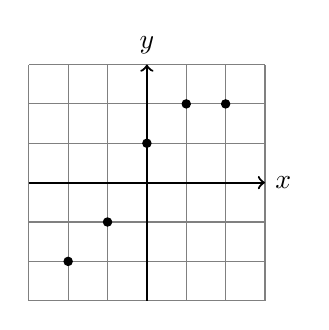
\begin{tikzpicture}[scale=0.5]
                \draw[gray] (-3,-3) grid (3,3); 
                \draw[->, thick]  (-3,0) -- (3,0)node [right] {$x$};
                \draw[->, thick]  (0,-3) -- (0,3)node [above] {$y$}; 
                \foreach \x/\y in {-2/-2,-1/-1,0/1,1/2,2/2} \filldraw (\x,\y) circle (.3em); 
    \end{tikzpicture}
    }
    \end{center}
    \end{minipage} 
    \onslide<4->{
    \vspace{12pt}
    \begin{center}
        Suppose we want to fit a straight line of the form $y = c_1 + c_2x$ to our data and need to determine $c_1$ and $c_2$. 
    \end{center}
    }
\end{frame}


\begin{frame}{Applying QR to Solve an Inconsistent System}
    \vspace{-6pt}
        \begin{center}
        \begin{tabular}{c|ccccc} 
            $ x$ & $-2$ & $-1$  & $0$ & $1$ & $2$ 
            \\ \hline 
            $ y$ & $-2$ & $-1$  & $1$ & $2$  & $2$
        \end{tabular}
    \end{center}
    Using the model $y=c_1 + c_2 x$, 
    \onslide<2->{
    $$A\vec x = \spalignmat{1 -2; 1 -1; 1 0 ; 1 1; 1 2 }\spalignmat{c_1;c_2}=\spalignmat{-2;-1;1;2;2}= \vec b$$}

    \vspace{2pt}
    \onslide<3->{We have a system of the form $A\vec x = \vec b$. To apply the QR decomposition, we need matrices $Q$ and $R$. }

\end{frame}






\begin{frame}{Example: Using QR to Solve Least-Squares}

    Compute the least-squares solution to $ A \vec x= \vec b$, where 
    \begin{equation*}
    A = 
    \spalignmat{1 -2; 1 -1; 1 0 ; 1 1; 1 2 }
    , \qquad 
    \vec b = 
    \spalignmat{-2;-1;1;2;2}
    \end{equation*}
\end{frame}













\begin{frame}{Example: Using QR to Solve Least-Squares}

    
    Using Gram-Schmidt, the $ QR$ decomposition of $ A$ is 
    \begin{equation*}
    A= QR = \spalignmat{1/\sqrt{5} -2/\sqrt{10}; 1/\sqrt{5} -1/\sqrt{10}; 1/\sqrt{5} 0 ; 1/\sqrt{5} 1/\sqrt{10}; 1/\sqrt{5} 2/\sqrt{10} }
    \begin{pmatrix}
    \frac{5}{\sqrt 5} & 0  \\ 0 & \frac{10}{\sqrt{10}}  
    \end{pmatrix}
    \end{equation*}
    
    \vspace{1in} 
\end{frame}


\begin{frame}{Example: Using QR to Solve Least-Squares}

    
    Next we need to compute $Q^T \vec b$. 
    \pause 
    \begin{align*}
    Q ^{T} \vec b = 
    \spalignmat{1/\sqrt{5} 1/\sqrt{5} 1/\sqrt{5} 1/\sqrt{5} 1/\sqrt{5} ; -2/\sqrt{10} -1/\sqrt{10} 0  1/\sqrt{10} 2/\sqrt{10} }
    \spalignmat{-2;-1;1;2;2} 
    = \begin{pmatrix}
      2/\sqrt5 \\ 11/\sqrt{10}
    \end{pmatrix}
    \end{align*}
    \pause
    Finally, we solve $R \widehat x = Q^T \vec b$. \pause 
    \begin{align*}
        \begin{pmatrix}
        \frac{5}{\sqrt 5} & 0  \\ 0 & \frac{10}{\sqrt{10}}  
        \end{pmatrix} \widehat x = \begin{pmatrix}
          2/\sqrt5 \\ 11/\sqrt{10}
        \end{pmatrix}
        \quad \Rightarrow \quad 
        \widehat x = \spalignmat{2/5 ; 11/10}
    \end{align*}
    \pause
    Thus, our linear model is $y = \frac{2}{5} + \frac{11}{10}x$. 
\end{frame}




\begin{frame}{Example: Using QR to Solve Least-Squares}

    Our linear model is $y = \frac{2}{5} + \frac{11}{10}x$. 
        \begin{center}
        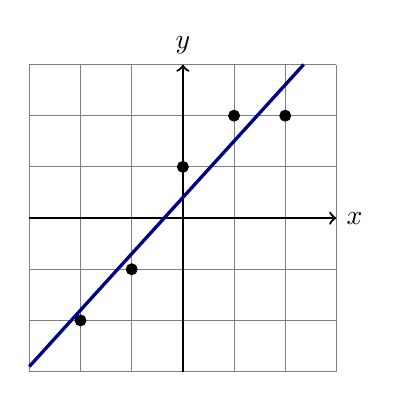
\begin{tikzpicture}[scale=0.65]
            \onslide<1->{
                \draw[gray] (-3,-3) grid (3,3); 
                \draw[->, thick]  (-3,0) -- (3,0)node [right] {$x$};
                \draw[->, thick]  (0,-3) -- (0,3)node [above] {$y$}; 
                \foreach \x/\y in {-2/-2,-1/-1,0/1,1/2,2/2} \filldraw (\x,\y) circle (.3em);
            }
            \onslide<2->{
                \draw[-,DarkBlue,very thick] (-3,-2.9) -- (2.36,3);
            }
        \end{tikzpicture}            
            
        \end{center}

    


\end{frame}


 \frame{\frametitle{Summary}

    \SummaryLine \vspace{4pt}
    \begin{itemize}\setlength{\itemsep}{8pt}

        \item using the QR decomposition to solve inconsistent linear systems 

    \end{itemize}
    
    \vspace{16pt}
    \pause 
    
    
}
